% Created 2021-03-12 Fri 14:19
% Intended LaTeX compiler: pdflatex
\documentclass[11pt]{article}
\usepackage[utf8]{inputenc}
\usepackage[T1]{fontenc}
\usepackage{graphicx}
\usepackage{grffile}
\usepackage{longtable}
\usepackage{wrapfig}
\usepackage{rotating}
\usepackage[normalem]{ulem}
\usepackage{amsmath}
\usepackage{textcomp}
\usepackage{amssymb}
\usepackage{capt-of}
\usepackage{hyperref}
\usepackage[top=1in, bottom=1.25in, left=1.25in, right=1.25in]{geometry}

\usepackage[main,include]{embedall}
\IfFileExists{./\jobname.org}{\embedfile[desc=The original file]{\jobname.org}}{}





\usepackage{fvextra}
\fvset{
  commandchars=\\\{\},
  highlightcolor=white!95!black!80!blue,
  breaklines=true,
  breaksymbol=\color{white!60!black}\tiny\ensuremath{\hookrightarrow},
}
\renewcommand\theFancyVerbLine{\footnotesize\color{black!40!white}\arabic{FancyVerbLine}}

\usepackage[many]{tcolorbox}
\DeclareTColorBox[]{Code}{}%
{enhanced,
  colback=white!97!black,
  colframe=white!94!black, boxrule=0.5pt,
  fontupper=\color{EFD}\footnotesize,
  arc=2.5pt, outer arc=2.5pt,
  boxsep=2pt, left=2pt, right=2pt, top=1pt, bottom=0.5pt,
  breakable}

\definecolor{EFD}{HTML}{383a42}
\definecolor{EFk}{HTML}{e45649}
\newcommand{\EFk}[1]{\textcolor{EFk}{#1}} % font-lock-keyword-face
\definecolor{EFd}{HTML}{84888b}
\newcommand{\EFd}[1]{\textcolor{EFd}{\textit{#1}}} % font-lock-doc-face
\definecolor{EFt}{HTML}{986801}
\newcommand{\EFt}[1]{\textcolor{EFt}{#1}} % font-lock-type-face
\definecolor{EFs}{HTML}{50a14f}
\newcommand{\EFs}[1]{\textcolor{EFs}{#1}} % font-lock-string-face
\definecolor{EFw}{HTML}{986801}
\newcommand{\EFw}[1]{\textcolor{EFw}{#1}} % font-lock-warning-face
\definecolor{EFb}{HTML}{a626a4}
\newcommand{\EFb}[1]{\textcolor{EFb}{#1}} % font-lock-builtin-face
\definecolor{EFct}{HTML}{9ca0a4}
\newcommand{\EFct}[1]{\textcolor{EFct}{#1}} % font-lock-comment-face
\definecolor{EFc}{HTML}{b751b6}
\newcommand{\EFc}[1]{\textcolor{EFc}{#1}} % font-lock-constant-face
\definecolor{EFpp}{HTML}{4078f2}
\newcommand{\EFpp}[1]{\textcolor{EFpp}{\textbf{#1}}} % font-lock-preprocessor-face
\definecolor{EFnc}{HTML}{4078f2}
\newcommand{\EFnc}[1]{\textcolor{EFnc}{\textbf{#1}}} % font-lock-negation-char-face
\definecolor{EFv}{HTML}{6a1868}
\newcommand{\EFv}[1]{\textcolor{EFv}{#1}} % font-lock-variable-name-face
\definecolor{EFf}{HTML}{a626a4}
\newcommand{\EFf}[1]{\textcolor{EFf}{#1}} % font-lock-function-name-face
\definecolor{EFcd}{HTML}{9ca0a4}
\newcommand{\EFcd}[1]{\textcolor{EFcd}{#1}} % font-lock-comment-delimiter-face
\definecolor{EFrc}{HTML}{4078f2}
\newcommand{\EFrc}[1]{\textcolor{EFrc}{\textbf{#1}}} % font-lock-regexp-grouping-construct
\definecolor{EFrb}{HTML}{4078f2}
\newcommand{\EFrb}[1]{\textcolor{EFrb}{\textbf{#1}}} % font-lock-regexp-grouping-backslash
\definecolor{EFhn}{HTML}{da8548}
\newcommand{\EFhn}[1]{\textcolor{EFhn}{\textbf{#1}}} % highlight-numbers-number
\definecolor{EFhq}{HTML}{4078f2}
\newcommand{\EFhq}[1]{\textcolor{EFhq}{#1}} % highlight-quoted-quote
\definecolor{EFhs}{HTML}{986801}
\newcommand{\EFhs}[1]{\textcolor{EFhs}{#1}} % highlight-quoted-symbol
\definecolor{EFrdi}{HTML}{4078f2}
\newcommand{\EFrdi}[1]{\textcolor{EFrdi}{#1}} % rainbow-delimiters-depth-1-face
\definecolor{EFrdii}{HTML}{a626a4}
\newcommand{\EFrdii}[1]{\textcolor{EFrdii}{#1}} % rainbow-delimiters-depth-2-face
\definecolor{EFrdiii}{HTML}{50a14f}
\newcommand{\EFrdiii}[1]{\textcolor{EFrdiii}{#1}} % rainbow-delimiters-depth-3-face
\definecolor{EFrdiv}{HTML}{da8548}
\newcommand{\EFrdiv}[1]{\textcolor{EFrdiv}{#1}} % rainbow-delimiters-depth-4-face
\definecolor{EFrdv}{HTML}{b751b6}
\newcommand{\EFrdv}[1]{\textcolor{EFrdv}{#1}} % rainbow-delimiters-depth-5-face
\definecolor{EFrdvi}{HTML}{986801}
\newcommand{\EFrdvi}[1]{\textcolor{EFrdvi}{#1}} % rainbow-delimiters-depth-6-face
\definecolor{EFrdvii}{HTML}{4db5bd}
\newcommand{\EFrdvii}[1]{\textcolor{EFrdvii}{#1}} % rainbow-delimiters-depth-7-face
\definecolor{EFrdiix}{HTML}{80a880}
\newcommand{\EFrdiix}[1]{\textcolor{EFrdiix}{#1}} % rainbow-delimiters-depth-8-face
\definecolor{EFrdix}{HTML}{887070}
\newcommand{\EFrdix}[1]{\textcolor{EFrdix}{#1}} % rainbow-delimiters-depth-9-face
\author{Jake Moss}
\date{\today}
\title{Chess piece position analysis}
\hypersetup{
 pdfauthor={Jake Moss},
 pdftitle={Chess piece position analysis},
 pdfkeywords={},
 pdfsubject={},
 pdfcreator={Emacs 28.0.50 (Org mode 9.5)}, 
 pdflang={English}}
\begin{document}

\maketitle

\section{What?}
\label{sec:org2d752c1}
This project aims to visualise a relationship between the positions of various
pieces and the players skill level. The positions of pieces, in states such as
captured, capturing, or checking, can be easily represented using an \texttt{8x8} heat
map. I also plan to present accompanying statistics utilising multi plots and
histograms of events through out a game.

A key plot I aim to produce is a multi plot with ranking on x-axis and piece
type on the y-axis. An example of this type of plot can be found \href{https://seaborn.pydata.org/\_images/axis\_grids\_18\_0.png}{here in the seaborn documentation}.

\section{Why?}
\label{sec:org3528091}
The purpose of this project is to show the positional differences between
different levels of play and over time. This is something not often visualised
within the community thus I thought it would be a unique take on some common
statistic.

\section{How?}
\label{sec:org54c9ee6}
Throughout this project I have been utilising a number of libraries such as
\texttt{numpy}, \texttt{matplotlib}, and \texttt{pandas} for general computation. Additionally I use
the \href{https://github.com/niklasf/python-chess}{python-chess} library to parse and interface with games on higher level.

For more general statistics I will adapt a \texttt{Chess.com} parsing script found
\href{https://public.tableau.com/views/MyChessJourney-Visualized/MyChessJourney?:language=en\&:display\_count=y\&publish=yes\&:origin=viz\_share\_link\&:showVizHome=no}{here}. An example of this script in action can be seen \href{https://public.tableau.com/views/MyChessJourney-Visualized/MyChessJourney?:language=en\&:display\_count=y\&publish=yes\&:origin=viz\_share\_link\&:showVizHome=no}{here}.

\section{Data source?}
\label{sec:org04ae696}
Chess games are found freely on the internet from many archives such as \href{https://www.pgnmentor.com/files.html}{PGN
Mentor}. From here I am able to download thousands of games at mass. However as
most games preserved will of famous players there will be significant bias. To
help mitigate this I can use the public API's from \href{https://lichess.org/}{Lichess} and \href{https://www.chess.com/}{Chess.com} to
gather games from friends and players from various ELO's.

To pull games from Chess.com I use this shell command to gather the PGN files
from individual months and write them to a single file as Chess.com does not
support downloading of all games at once.
\begin{Code}
\begin{Verbatim}[]
\color{EFD}\EFk{for} g\EFk{ in} \$\textcolor[HTML]{4078f2}{(}\textcolor[HTML]{986801}{curl} -Ls https://api.chess.com/pub/player/\$\EFv{PLAYERNAME}/games/archives | jq -rc \EFs{".archives[]"}\textcolor[HTML]{4078f2}{)} ; \EFk{do} \textcolor[HTML]{986801}{curl} -Ls \EFs{"}\textcolor[HTML]{b751b6}{\$}\textcolor[HTML]{6a1868}{g}\EFs{"} | jq -rc \EFs{".games[].pgn"} ; \EFk{done} >> games.pgn
\end{Verbatim}
\end{Code}

Lichess easily allows for downloading of an entire players archive at once with
a simple \texttt{curl}.
\begin{Code}
\begin{Verbatim}[]
\color{EFD}\textcolor[HTML]{986801}{curl} https://lichess.org/games/export/\$\EFv{PLAYERNAME} > games.pgn
\end{Verbatim}
\end{Code}

\section{Examples}
\label{sec:org7aaad79}
\begin{Code}
\begin{Verbatim}[]
\color{EFD}\EFk{import} chess
\EFk{import} chess.pgn
\EFk{import} chessHeatmap
\end{Verbatim}
\end{Code}

\begin{Code}
\begin{Verbatim}[]
\color{EFD}\EFv{pgn} = chessHeatmap.load\_pgn(\EFs{"Dae.pgn"})

\EFv{filename\_pawn} = chessHeatmap.lost\_piece\_plot(pgn, [chess.PAWN])
filename\_pawn
\end{Verbatim}
\end{Code}

\begin{figure}[htbp]
\centering
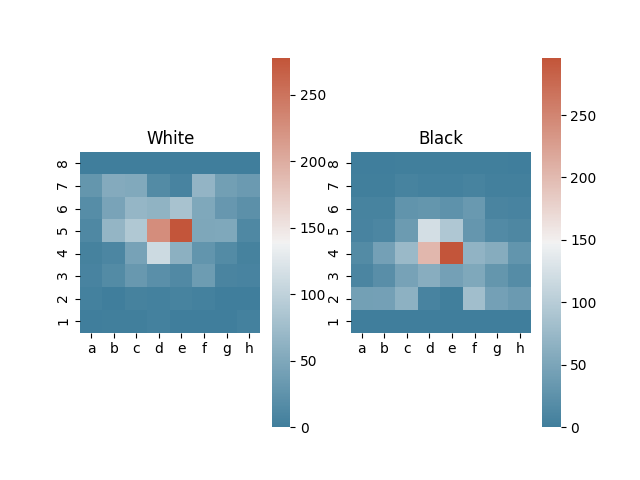
\includegraphics[width=.9\linewidth]{DaenaliaEvandruile_Lost_piece_plot__pawn.png}
\caption{Pawns lost from whites POV}
\end{figure}

\newpage

\begin{Code}
\begin{Verbatim}[]
\color{EFD}\EFv{filename\_knight} = chessHeatmap.lost\_piece\_plot(pgn, [chess.KNIGHT])
filename\_knight
\end{Verbatim}
\end{Code}

\begin{figure}[htbp]
\centering
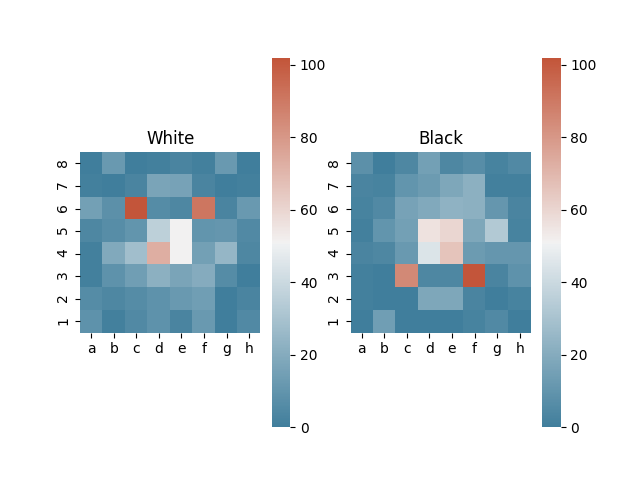
\includegraphics[width=.9\linewidth]{DaenaliaEvandruile_Lost_piece_plot__knight.png}
\caption{Knights lost from whites POV}
\end{figure}
\end{document}
